\documentclass{article}

% CS230 project milestone template, built on the official NeurIPS 2026 style file.
% Keep the [final] option: it prints the author block and omits line numbers.
\PassOptionsToPackage{numbers,compress}{natbib}
\usepackage[final]{neurips_2026}

\usepackage[utf8]{inputenc} % allow utf-8 input
\usepackage[T1]{fontenc}    % use 8-bit T1 fonts
\usepackage{hyperref}       % hyperlinks
\usepackage{url}            % simple URL typesetting
\usepackage{booktabs}       % professional-quality tables
\usepackage{amsfonts}       % blackboard math symbols
\usepackage{amsmath}        % \operatorname, align
\usepackage{nicefrac}       % compact symbols for 1/2, etc.
\usepackage{microtype}      % microtypography
\usepackage{xcolor}         % colors
\usepackage{graphicx}       % figures
\newcommand{\pagelimit}{3}

\title{Skier Tracking and 2D Body-and-Ski Landmark Estimation}

\author{%
  Ruichao Zhang \\
  \texttt{ruichaoz@stanford.edu} \\
}

\begin{document}

\maketitle

\section{Introduction}
Reviewing a ski run on video is hard: broadcast cameras pan and zoom, the skier is small and often hidden by
gates, and the skis are thin, fast, overlapping objects that general-purpose pose models do not predict at all. We
build a pipeline for visual movement review. \textbf{The input is a single-camera skiing video and a box around the
skier in the first frame.} A fixed, pretrained SiamFC tracker~\cite{bertinetto2016fully} follows the skier; a
COCO-pretrained HRNet-W32~\cite{sun2019deep,lin2014microsoft} fine-tuned to 24 landmarks (14 body, 8 ski, 2 pole)
\textbf{outputs 2D landmarks} on crops cut around the tracker box; and a geometric controller turns the tracker boxes
into a smooth, skier-centered replay with the skeleton drawn on it. Plain fine-tuning is our baseline, not our
contribution. Our contributions are: (1) a new task for a pretrained pose model, body plus ski and pole landmarks,
which COCO models cannot predict, on crops cut around a tracker box instead of the labels; (2) tracker-aware
training, a controlled study of targeted augmentation (crop jitter that mimics tracker box error, motion blur,
synthetic occlusion) against plain fine-tuning, with paired seeds and a selection rule fixed in advance; (3)
pose-guided crop refinement, a second prediction on a crop around the first one, which recovers a third of the ski
accuracy lost to tracker crops; and (4) a measurement of how much tracking error costs pose accuracy downstream,
with a confidence-gated replay that stays usable when the tracker fails. The topic is unchanged from the proposal; Section~\ref{sec:approach} lists the small
changes.

\section{Dataset}
\textbf{Ski 2DPose}~\cite{bachmann2019motion} has 1,982 images from 16 alpine skiing videos (Creative-Commons YouTube
sources; the dataset page states no separate annotation license), labeled at sparse frames of 158 single-camera
segments with 24 landmarks and visibility flags. We split by source video so that no video crosses partitions: train
4 videos / 1,194 images, val 3 / 293, test 3 / 360. The 6 follow-cam videos (134 images, a different camera setup)
are a separate set evaluated once at the end, and 1 record with fewer than two reliable points is excluded. Only
visible labels are supervised and scored (val: 3,759 body and 1,752 ski labels). Each of the 293 val images is
best matched by its own video frame, which the integration experiment needs. \textbf{SkiTB}~\cite{dunnhofer2024tracking} (CC BY-NC 4.0) provides skier boxes for 100
alpine sequences. We use its official athlete-disjoint split (53/6/41 sequences) and its single-camera clips: 75 val
clips (12,925 scored frames) and 471 test clips. Frame rates are not stored, so we estimate them per sequence (25 or
30 fps) from frame span and official race time.

\textbf{Preprocessing.} The reference box is the tight box around the reliable body and ski points. It is padded by
1.25, fitted to 3:4 and warped to a $256\times192$ crop with ImageNet normalization; targets are $64\times48$ heatmaps
with sub-pixel Gaussians ($\sigma=2$). Standard augmentation: horizontal flip ($p=0.5$, left/right labels swapped),
rotation $\pm15^\circ$, scale 0.8--1.2.

\section{Approach}\label{sec:approach}
\textbf{Model and loss.} We load MMPose's~\cite{mmpose2020} COCO-pretrained HRNet-W32 and replace its last
$1\times1$ layer to output $K=24$ heatmaps. With $\hat H_{ij}$ and $H_{ij}$ the predicted and target heatmaps of
landmark $j$ in sample $i$, and $v_{ij}=1$ for a visible label inside the crop (else 0), we minimize the masked
mean-squared error
\[
\mathcal{L} = \frac{\sum_{i,j} v_{ij}\, \operatorname{mean}_{u,v}\big(\hat H_{ij}(u,v) - H_{ij}(u,v)\big)^2}
{\max\big(1, \sum_{i,j} v_{ij}\big)} .
\]
Decoding follows MMPose; our pipeline matches MMPose's own inference to 0.014\,px on average.

\textbf{Training.} Adam~\cite{kingma2015adam}, batch 16: 3 warm-up epochs with the backbone frozen (head learning rate
$10^{-3}$), then 150 fine-tune epochs at $10^{-4}$ (backbone) and $5\times10^{-4}$ (head), multiplied by 0.1 at
fine-tune epochs 90 and 127. We keep the checkpoint with the best val ski PCK. Each recipe is trained with two seeds;
within a seed, all recipes see identical data order, flips, rotations and scales, so they differ only in the added
augmentation.

\textbf{Baselines and experiments.} \emph{E0}: the unchanged COCO model, scored on the 10 body landmarks COCO shares
with our schema (it cannot predict skis). \emph{E1}: fine-tuning with standard augmentation, our main baseline.
\emph{E2}: E1 + crop jitter (box center shifted by up to $\pm10\%$ per axis, size $\times$0.9--1.1), which mimics
tracker error. \emph{E3}: E1 + motion blur ($p=0.5$, line kernel 3--9\,px) and a random occluding patch ($p=0.5$,
5--15\% of the crop). \emph{E4}: all three. A rule fixed before any E2--E4 result picks the recipe: the highest val
ski PCK@0.1 among recipes that lose at most 2 points of body PCK. Ties (within 1 point) go to the higher ski PCK on a
fixed val \emph{crop-error set}, where reference boxes are shifted and rescaled by 5/10/20\% of their size.

\textbf{Metrics.} PCK@$t$ is the share of visible labels predicted within $t$ times the reference-box diagonal; we
report body and ski separately (poles are supplementary), and a missing prediction counts as a miss. The two seeds
are pooled by summing hits and totals. Labeled frames within a segment are strongly correlated, so 95\% intervals
come from a cluster bootstrap~\cite{efron1994introduction} that resamples segments within each video (10,000
resamples); tracking intervals resample SkiTB sequences.

\textbf{Tracking, replay and integration.} SiamFC with GOT-10k-pretrained weights~\cite{huang2019got} is initialized
once per clip. Its confidence is the peak of its normalized response map. On SkiTB val it predicts failure frames
(IoU\,$<$\,0.1) with ROC AUC 0.83, and frames below a threshold set by Youden's $J$ on val are flagged as
low-confidence. The replay crop is the tracker box enlarged $2.5\times$ and fitted to 16:9, then smoothed
exponentially with a 0.2\,s time constant; on flagged frames it holds its center and zooms out. In the integration
experiment, the tracker starts at a segment's first labeled frame with its reference box. At every later labeled
frame, the same model runs on the reference crop and on a crop around the tracker box ($1.1\times$, chosen on val),
and both are scored against the same labels. Every setting was chosen on val by a rule written down before its run.

\textbf{Pose-guided crop refinement.} A tracker box that only partly covers the skier gives a badly framed crop, but
the model often still finds the body in it. We therefore predict twice: the tight box around the first-pass body
and ski landmarks with heatmap score at least $s_{\min}$, enlarged by $k_{\mathrm{ref}}$, is cropped like a training
crop and predicted again; with fewer than 4 such landmarks the first pass is kept. It uses no labels and no
retraining. A rule fixed before the run chose $s_{\min}=0.3$ and $k_{\mathrm{ref}}=1.3$ from 12 settings on val.

\textbf{Changes since the proposal.} (i) Two seeds per recipe instead of three. (ii) 150 fine-tune epochs instead of
50, after the convergence problem described in Section~\ref{sec:results}. (iii) A 65/16/19 split by video, with the
follow-cam videos set aside. (iv) The stretch goals (amateur footage, 3D, coaching) are dropped. (v) Crop
refinement is new.

\paragraph{Remaining work.} (1) After TA feedback, by Nov 15: freeze code, configurations and checkpoints (hashes
recorded) and evaluate the test set \emph{once}: pose (E0, E1, E2), the follow-cam set, tracking with our metrics and
the SkiTB toolkit's official F-score, the replay, and the integration experiment with and without crop refinement,
all with the same intervals. The evaluation script is written and has passed a full dry run on val. (2) Optionally,
replace SiamFC with an off-the-shelf STARK tracker~\cite{yan2021learning}, adopted only if it is better on val.
(3) Final report: test
tables, failure analysis, and 2--3 demo clips, including a failure.

\section{Partial Results}\label{sec:results}
All numbers are on the val partition (held out from training); test has not been touched.

\begin{table}[h]
  \centering
  \small
  \begin{tabular}{llcccc}
    \toprule
    & Added augmentation & Body @0.1 & Ski @0.1 & Ski @0.05 & Ski @0.1, crop error$^{\dagger}$ \\
    \midrule
    E0 & none (COCO, not fine-tuned) & 95.1$^{*}$ & -- & -- & -- \\
    E1 & none (baseline) & 95.2 & 91.9 & 82.9 & 90.4 \\
    E2 & crop jitter & 95.5 & \textbf{93.1} & \textbf{84.3} & \textbf{92.9} \\
    E3 & blur + occlusion & 96.9 & 92.0 & 82.0 & 90.9 \\
    E4 & all three & \textbf{97.1} & 91.0 & 78.8 & 89.5 \\
    \bottomrule
  \end{tabular}
  \caption{Pose accuracy on val, PCK (\%), mean of two seeds; 3,759 body and 1,752 ski labels per seed.
  $^{*}$E0 is scored on the 10 body landmarks shared with COCO (E1 on the same subset: 95.5).
  $^{\dagger}$The moderate level of the fixed crop-error set (boxes shifted by 10\% of their size).}
  \label{tab:pose}
\end{table}

\textbf{Fine-tuning and augmentation (Table~\ref{tab:pose}).} Fine-tuning (E1) matches the COCO model on the shared
body landmarks at PCK@0.1 ($+0.4$ points, 95\% CI $[-1.2, 1.7]$), is clearly more precise at PCK@0.05 ($+4.6$,
$[2.4, 6.7]$), and adds ski landmarks at 91.9\%. Of the augmentations, only crop jitter (E2) improves the skis: $+1.2$
points at PCK@0.1 ($[0.1, 2.3]$), $+1.5$ at 0.05 ($[0.4, 2.6]$), and $+2.5$ on moderately mis-centered crops
($[1.5, 3.6]$), with body PCK unchanged ($+0.3$, $[-0.7, 1.2]$). Blur and occlusion (E3, E4) raise body PCK by
1.7--1.9 points but not ski PCK. The pre-registered rule picks E2, on the seed means and on each seed alone. The gain
falls short of the 5 points we aimed for. Because val also selects each run's best epoch, val numbers are slightly
optimistic for all runs alike; test will give unbiased ones.

\textbf{An assumption that did not hold.} We first trained for 50 fine-tune epochs. E2--E4 then reached only 69--78\%
val ski PCK against E1's 89.5\%, which looked like augmentation hurting the skis. A per-landmark analysis showed
instead that the ski \emph{tails} were not learned at all, even on the training images (about 20\% vs.\ 73--78\% for
E1), and that E1 itself failed the same way with another seed (69.4\%). Ski tails are learned late, around fine-tune
epochs 60--80. We therefore reran every recipe for 150 epochs with two seeds. All eight runs then learn the tails
(at least 77\% on the training images), and Table~\ref{tab:pose} uses these runs.

\begin{table}[h]
  \centering
  \small
  \begin{tabular}{p{0.27\linewidth}p{0.66\linewidth}}
    \toprule
    SiamFC, SkiTB val (75 clips) & pooled IoU 0.363 [0.299, 0.453]; toolkit F-score 0.384; 40 clips lose the skier
    for $\geq$0.5\,s \\
    Replay & skier box fully inside the crop in 89\% of SkiTB frames; ski ends inside on Ski 2DPose: 99.4\%
    (834/839); acceleration $2.6\times$ lower \\
    E2, reference $\to$ tracker crop & body 95.9 $\to$ 81.1, ski 93.8 $\to$ 75.4 (PCK@0.1; 261 labels, 31 segments) \\
    E2, refined tracker crop & body 83.9, ski 81.3 (over the tracker crop: body $+2.8$ $[1.2, 4.5]$, ski $+5.9$
    $[3.6, 8.4]$) \\
    \bottomrule
  \end{tabular}
  \caption{The integrated system on val. Replay acceleration is relative to an unsmoothed crop.}
  \label{tab:system}
\end{table}

\begin{figure}[h]
  \centering
  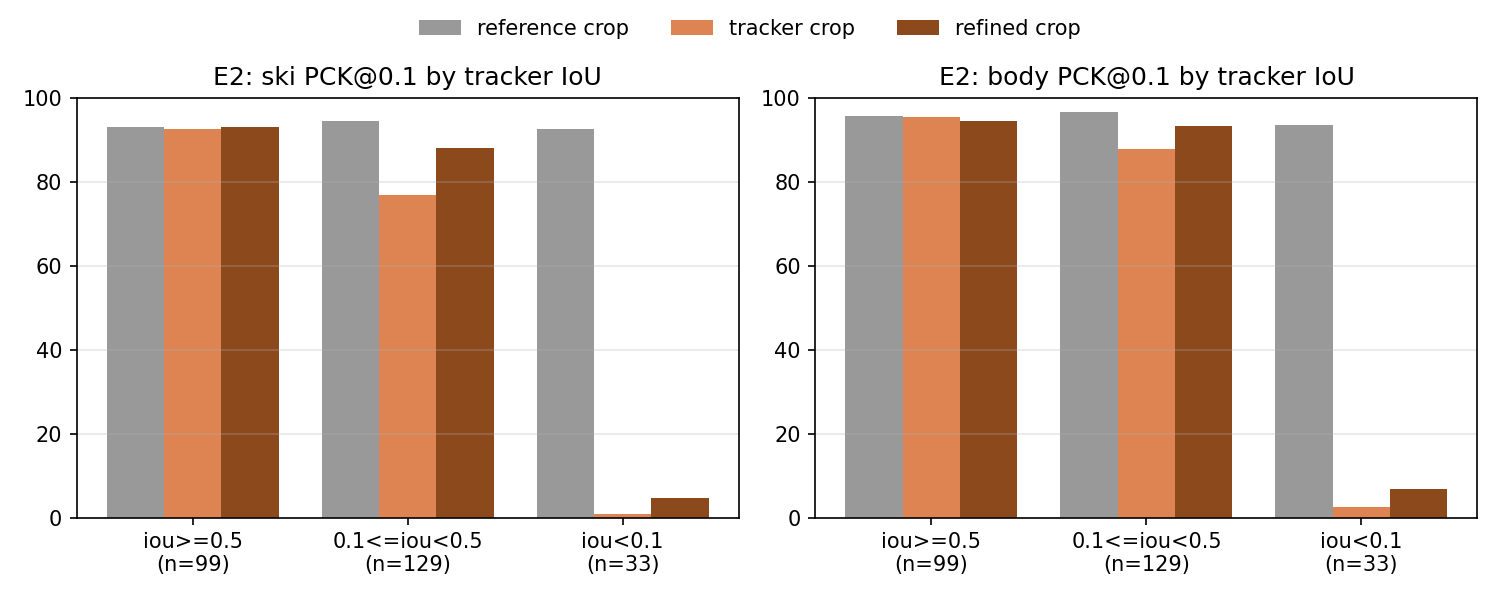
\includegraphics[width=0.7\linewidth]{figures/propagation_strata_val.png}
  \caption{E2 pose accuracy from reference crops (grey), tracker crops (orange) and refined tracker crops (brown) on
  val, grouped by the IoU between the tracker box and the reference box.}
  \label{fig:strata}
\end{figure}

\textbf{The integrated system (Table~\ref{tab:system}, Figure~\ref{fig:strata}).} SiamFC is the weak link: it loses
the skier for at least 0.5\,s in 40 of 75 clips, drifting to spectators, banners or on-screen graphics. The replay is
still usable, because flagged frames zoom out: 99.4\% of ski endpoints stay inside the crop, above our 95\% target.
Pose suffers more. Cropping around the tracker box instead of the labels costs E2 14.8 body and 18.4 ski points
($[12.5, 25.2]$). When the tracker box overlaps the reference box with IoU\,$\geq$\,0.5 there is no loss (ski 93.2 $\to$
92.5), so the drop comes from tracker drift, not from a mismatch between training and inference crops. Crop jitter
pays off here: under tracker crops, E2 beats E1 by 2.4 ski points ($[1.3, 3.5]$). Crop refinement recovers about a
third of the loss: ski 75.4 $\to$ 81.3 and body 81.1 $\to$ 83.9. On partly overlapping boxes (IoU 0.1--0.5, 129
labels) ski PCK rises from 76.8 to 88.0, where the box was already good it stays level (92.5 $\to$ 93.1), and it
cannot help once the skier is lost (IoU\,$<$\,0.1: 0.9 $\to$ 4.6). Refinement and crop jitter fix the same
mis-framing, so after refinement E2 leads E1 by only 1.3 ski points ($[-0.9, 3.0]$). The confidence flag separates bad
frames (ski PCK 57.9\% on flagged vs.\ 81.8\% on other labels), and the overlay is hidden on them. The tracker is
therefore the main lever for the final system, which motivates the optional STARK experiment.

\section*{References}
\renewcommand{\bibsection}{}   % the "References" heading is already typeset above
\medskip
{\small
\bibliographystyle{plainnat}
\bibliography{references}
}

\end{document}
